\documentclass[a4,center,fleqn]{NAR}


\usepackage{NAR-natbib}
\bibliographystyle{unsrtnat}
\usepackage{color}
\usepackage{xfrac}
\newcommand{\rngcomment}[1]{{\color{red}RNG: #1}}
\newcommand{\bkmcomment}[1]{{\color{blue}BKM: #1}}
\newcommand{\batcave}{BATCAVE }
% Enter dates of publication
\copyrightyear{2008}
\pubdate{31 July 2009}
\pubyear{2009}
\jvolume{37}
\jissue{12}

\articlesubtype{Genomics and Bioinformatics}

\begin{document}

\title{\batcave: Bayesian Analysis Tools for Context-Aware Variant Evaluation}

\author{%
Brian K. Mannakee\,$^{1}$ and
Ryan N. Gutenkunst\,$^{2}$%
\footnote{To whom correspondence should be addressed.
Email: rgutenk@email.arizona.edu}}

\address{%
$^{1}$Mel and Enid Zuckerman College of Public Health, University of Arizona, Tucson AZ
and
$^{2}$Department of Molecular and Cellular Biology, University of Arizona, Tucson AZ}
% Affiliation must include:
% Department name, institution name, full road and district address,
% state, Zip or postal code, country

\history{%
Received January 1, 2009;
Revised February 1, 2009;
Accepted March 1, 2009}

\maketitle

\begin{abstract}
Text. Text. Text. Text. Text. Text. Text. Text. Text. Text. Text.
Text. Text. Text. Text. Text. Text. Text. Text. Text. Text. Text.
Text. Text. Text. Text. Text. Text. Text. Text. Text. Text. Text.
Text. Text. Text. Text. Text. Text. Text. Text. Text. Text. Text.
Text. Text. Text. Text. Text. Text. Text. Text. Text. Text. Text.
Text. Text. Text. Text. Text. Text. Text. Text. Text. Text. Text.
Text. Text. Text. Text. Text. Text. Text. Text. Text. Text. Text.
Text. Text. Text. Text. Text. Text. Text. Text. Text. Text. Text.
Text. Text.
\end{abstract}


\section{Introduction}

Cancer develops as the result of the accumulation of somatic mutations and clonal selection of cells with mutations that confer a selective advantage on the cell.
Understanding the forces that shaped the evolutionary history of a tumor, the mutations that are responsible for its growth, the rate at which mutations are occurring, or how much genetic diversity is likely present in the tumor, requires accurate variant calling, particularly at low variant allele frequency \cite{Williams2016,Bozic2016,Williams2018}.
Accurate variant identification is also critical in optimizing the treatment regime for an individual patients disease \citep{Ding2012,Mardis2012,Chen2013,Borad2014,Findlay2016}.
Low frequency mutations present a significant problem for current mutation calling methods because their signature in the data is difficult to distinguish from the noise introduced by Next Generation Sequencing (NGS), and this problem increases as sequencing depth increases.

Methods for identifying true somatic mutations - i.e. variant calling -  from NGS data are an active area of research in bioinformatics.
The earliest widely used somatic variant callers aimed specifically at tumors, Mutect1 and Varscan2, used a combination of heuristic filtering and a model of sequencing errors to identify and score potential variants, setting a threshold for that score designed to balance sensitivity and specificity \citep{Koboldt2012,Cibulskis2013}.
Subsequent research gave rise to a number of alternate variant calling strategies including haplotype based callers \citep{Garrison2012},
joint genotype analysis (SomaticSniper, JointSNVMix2, Seurat, and CaVEMan,MuClone)\citep{Larson2012,Roth2012a,Christoforides2013,Jones2016,Dorri2019}, allele frequency based analysis (Strelka, MuTect, LoFreq, EBCall, deepSNV, LoLoPicker, and MuSE)\citep{Saunders2012,Wilm2012,Shiraishi2013b,Gerstung2012,Carrot-Zhang2017,Fan2016}, and a mixture of ensemble and deep learning methods (MutationSeq, SomaticSeq, SNooPer, and BAYSIC).
All of these methods have varying levels of complexity, and some are focused on specific types of data.
The one thing they all have in common is that they either implicitly or explicitly assume that the probability of a mutation occuring at a particular site is proportional to the overall mutation rate, and the same at every site in the genome.

Single nucleotide substitions, i.e. simple mutations, arise in tumors at a rate and at genomic locations driven by two main processes. 
The first is the spontaneous accumulation of mutations that occurs in all dividing tissues, and has a characteristic mutation signature that describes the probability of mutation in a given genomic context \citep{Nik-Zainal2012a,Alexandrov2015,Lee-Six2018}. 
The second, and far more complex, process is the accumulation of mutations through exposure to mutagens or degradation - via mutation or deletion - of cellular machinery responsible for the identification and repair of damage or replication errors. 
Many mutagens and DNA repair mechanism defects also have highly specific mutation signatures, such that they can be identified by observing the mutations in the tumor \citep{Alexandrov2013a,Helleday2014a,Nik-Zainal2016,Kandoth2013,Alexandrov2016}.

Here we present an algorithm for estimating the prior probability of mutation at a given site using the observed mutation spectrum of the tumor as well as its mutation rate, and show that the addition of this prior to the MuTect variant calling model produces a superior variant classifier in both simulated and real tumor data.
We then extend the method with an application of the local false discovery rate by computing the probability that a site is non-null under an assumption of clonal expansion with either early or small selective differences between clones.
We provide a simple implementation in R that takes MuTect caller output as input, and returns the posterior probability that a site is variant for every site observed by MuTect. \bkmcomment{batcave,batcaver,batcaveR}

\section{MATERIALS AND METHODS}
\subsection{Somatic variant calling base probability model}

At every site in the genome with non-zero coverage, Next Generation Sequencing (NGS) produces a vector $\mathbf{x}  = (\{b_i\},\{q_i\}), i = 1\dots \mathrm{d}$ of base calls and their associated quality scores, where $\mathrm{d}$ is total read depth.
We want to use $\mathbf{x}$ to select between competing hypotheses;
$$
  \begin{array}{l}
    \mathbf{H_0}:\quad \textrm{Alt allele} = m;\quad\nu = 0\\
    \mathbf{H_1}:\quad \textrm{Alt allele} = m;\quad\nu = \hat{f},
  \end{array}
$$
where $\nu$ is the variant allele frequency, $\hat{f}$ is the maximum likelihood estimate of $\nu$ given data $\mathbf{x}$, i.e. the ratio of the count of variant reads and total read depth, and $m$ is any of the 3 possible alternate non-reference bases.
The posterior probability of a given hypothesis, $P(m,\nu)$, is the product of the likelihood of the data given the hypothesis and the prior probability of the hypothesis. 
Assuming that reads are independent, we have

\begin{equation}
  \label{eqn:1}
$$
  P(m,\nu) = p(m,\nu) \cdot \prod_{i=1}^{\mathrm{d}} \textrm{f}_{m,\nu}(x_i),
$$
\end{equation}
where the density $\textrm{f}_{m,\nu}(x_i)$ can take several forms.

Assuming that the identity of the alternate allele and its allele frequency are independent of each other, and $\nu$ is uniformly distributed (i.e. $p(\nu) = 1$), we can rewrite equation \ref{eqn:1} as
\begin{equation}
  \label{eqn:2}
$$
  P(m,\nu) = p(m) \cdot \prod_{i=1}^{D} \textrm{f}_{m,\nu}(x_i).
$$
\end{equation}
Here we show how \batcave can be used to provide a tumor-specific estimate of the mutation probability $p(m)$.

\subsection{Site-specific prior probability of mutation}
The probability which we have denoted $p(m)$ in equation \ref{eqn:2} for compactness is more precisely the joint probability that a mutation has occured $M$, and that it was to allele $m$, which we will denote here $p(m,M)$.
However, $p(m,M)$ is not constant for every site in the genome, and follows a distribution conditional on the genomic context surrounding the site, denoted here $p(m,M | C)$ \cite{Buisson2019}.
Assuming that $m$ and $M$ are independent conditional on the genomic context, $\mathrm{p}(m,M \mid C) = \mathrm{p}(m \mid C) \mathrm{p}(M \mid C)$, which we can use Bayes' rule to further decompose as 

\begin{equation}
  \label{eqn:full_prior}
  $$
  \mathrm{p}(m,M \mid C) = \mathrm{p}(m \mid C) \mathrm{p}(C \mid M)\frac{p(M)}{p(C)}.
  $$
\end{equation}
We next show how to estimate the quantities in equation \ref{eqn:full_prior}.

\subsection{Estimation of the mutation profile}
There are many aspects of genomic architecture which can affect the somatic mutation rate at multiple scales \cite{Buisson2019}.
Here we focus on a small-scale feature, the tri-nucleotide context, which has been shown to have a strong effect on the prior probability of mutation \citep{Nik-Zainal2012a,Alexandrov2015,Lee-Six2018}.
The tri-nucleotide context at a particular genomic site is made up of the identity of the reference base and the identity of the 3` and 5` flanking bases.
There are four possible bases {\{A,C,T,G\}} 3` and 5` of the site, leading to 16 possible flanking base combinations.
Folding the central bases to the pyrimidines leaves 2 possible reference bases at the site {\{C,T\}}, resulting in $2 \cdot 16 = 32$ possible tri-nucleotide contexts.
We define a mutation context $C$ indexed by $i=\{1 \dots 32\}$, to be the tri-nucleotide context of a particular site in the genome. 
For each context, a mutation can be to any of the three possible alternate alleles {\{A,(C/T),G\}}. 
We can thus define $\mathrm{S}$, the substitution type, indexed by $i=\{1 \dots 32\}$ contexts and $j = \{1 \dots 3\}$ alternate bases, resulting in 96 possible substitution types.
Using the substitution type $\mathrm{S}$, we can rewrite equation \ref{eqn:full_prior} as 

\begin{equation}
  \label{eqn:detailed_prior}
  $$
  \begin{array}{rcc}
  \mathrm{p}(\mathrm{S}) &=&  \mathrm{p}(m =j, M | C = i) \\
                            &=& \mathrm{p}(m = j \mid C = i) \mathrm{p}(C = i \mid M)\frac{p(M)}{p(C = i)},
  \end{array}
  $$
\end{equation}
where $\mathrm{p}(\mathrm{S})$ is the probability that a substitution of type $S$ has occurred.

\begin{figure}[t]
  \begin{center}
  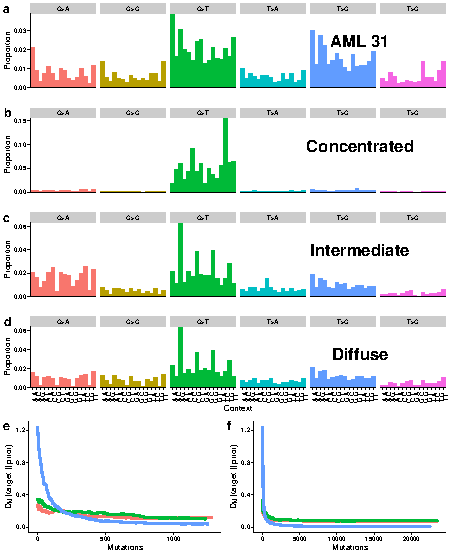
\includegraphics{figures/signature_figure.pdf}
  \end{center}
  \caption{Mutation profiles. 
  \textbf{(a)} The observed mutation profile of a breast cancer sample from \cite{Shi2018}.
  \textbf{(b)} The observed mutation profile of the AML 31 primary tumor from \cite{Griffith2015}.
  \textbf{(c)} A mutation profile used for simulating tumors, made up of equal proportions of COSMIC mutation signatures 1, 7, \& 11.
  \textbf{(d)} Equal proportions of signatures 1, 4, \& 5.
  \textbf{(e)} Equal proportions of signatures 1, 3, \& 5.
  KL divergence between the estimated profile ($\boldsymbol{\pi}$) and the simulated mutation profile for \textbf{(f)} Whole exomes and \textbf{(g)} whole genomes.
  The estimated mutation profile converges quickly to the target as the number of mutations evaluated rises.
  }
  \label{NAR-sigfig}
  \end{figure}

Figure \ref{NAR-sigfig} \textbf{a-e} shows several examples of mutation profiles from both real and simulated tumors.
The mutation profiles in Figure \ref{NAR-sigfig} can be described compactly by the vector $\boldsymbol{\pi}$ where each element of $\boldsymbol{\pi}$ represents the proportion of all observed tumor mutations of substitution type $\mathrm{S}_{i,j}$.
The distribution of observed substitutions $ \mathrm{p}(\mathrm{S}) $, is multinomial with parameter $ \boldsymbol{ \pi } = \{\pi_{i,j}\} $.
In a tumor with a very large number of verified mutations $\boldsymbol{\pi}$ could be estimated directly from the observed mutation profile, but in practice we find that many elements of $\boldsymbol{\pi}$ will have $0$ or a very small number of mutations present in the tumor.
As a result we need to model $p(S)$ as dirichlet - multinomial with pseudo-count hyper-parameter $\boldsymbol{\alpha}$, 

$$
\begin{aligned}
  \boldsymbol{\pi} \mid \boldsymbol{\alpha} &\sim \textrm{Dirichlet}(\boldsymbol{\alpha}) \\
  S \mid \boldsymbol{\pi} & \sim \textrm{Multinomial}(\boldsymbol{\pi}).
\end{aligned}
$$
In \batcave we use the symmetric non-informative hyper-parameter $\boldsymbol{\alpha} = \boldsymbol{1}$, so a-priori a mutation is equally likely in any context.

\bkmcomment{Introduce D earlier as its own section describing how we get it? Or expound here instead.}

Let $\mathrm{D}$ be the set of high confidence variant calls, and $c \in \mathrm{D}$ be the context of each mutation in $\mathrm{D}$.
The posterior distribution of $\boldsymbol{\pi}$ is then $\mathrm{p}(\boldsymbol{\pi} \mid \mathrm{D}) \sim \textrm{Dirichlet}(\boldsymbol{\alpha^{\prime}})$ where
  $$
    \alpha^{\prime}_{i,j} = \alpha_{i,j} + \sum\limits_{c \in \mathrm{D}} \mathrm{I}\{c = c_{i,}\}.
  $$
Returning to equation \ref{eqn:detailed_prior}, we can compute the posterior predictive probability $p(C_{i} \mid M,\mathrm{D})$ as
\begin{equation}
  \label{eqn:post_pred}
  $$
  p(C = C_{i} \mid M,\mathrm{D}) = \frac{\sum_{j}\alpha^{\prime}_{i,j}}{\sum_{i,j}\alpha^{\prime}_{i,j}}.
  $$
\end{equation}
The posterior probability of mutation to allele $m$ given that a mutation has occurred in context $C_{i}$, $p(m = j \mid C_{i},\mathrm{D})$ is then
\begin{equation}
  \label{eqn:to_allele}
  $$
   p(m = j \mid C_{i},\mathrm{D}) = \frac{\alpha^{\prime}_{i,j}}{\sum_{j} \alpha^{\prime}_{i,j}}.
  $$
\end{equation}
The remaining context dependent component in equation \ref{eqn:full_prior} is $p(C = C_{i})$, the prior probability of seeing a particular tri-nucleotide context.
We compute this as simply the proportion of all tri-nucleotide contexts with the context $C_{i}$ present in the genome.
\bkmcomment{I have a pre-computed table in batcaver for wes and wgs. Should I add that bit here?}

\subsection{Estimation of the mutation rate.}
The final piece of equation \ref{eqn:full_prior} to specify is $p(M)$, the prior probability that a mutation will occur at a given site, which usually specified as the mutation \textit{rate} per base $\mu$.
In an exponentially growing tumor, the number of new mutations per cell division is the product of the number of bases $N$, the per base mutation rate $\mu$, and the \textit{effective} birth rate $\beta$, which is a function of the birth $b$ and death $d$ rates.
\citet{Williams2016} showed that if 
$$
  \beta = \frac{b-d}{b},
$$
then the number of new mutations per cell division is
$$
  \frac{N \mu}{\beta}.
$$
In a neutrally or nearly neutrally evolving tumor, they further show that the total number of mutations $\mathrm{M}$ between two allele frequencies ($f_{min}$,$f_{max}$) is
\begin{equation}
  \label{eqn:mut_rate}
$$
  \mathrm{M}(f_{min},f_{max}) = N\frac{\mu}{\beta}\left(\frac{1}{f_{min}} - \frac{1}{f_{max}}\right).
$$
\end{equation}
\bkmcomment{Gets weaker here in terms of how this needs to be said and how much of it needs to be said. Need to decide where to add the factor of two.}

The number of bases $N$ is fixed at $3\cdot10^9$ for a whole genome sequence and $3\cdot10^7$ for a whole exome.
Returning to the set of high confidence mutations $\mathrm{D}$, we can set $f_{max}$ to be the largest allele frequency in $\mathrm{D}$, $f_{min}$ as the lowest, and count the number of mutations in $D$ falling between the two.
In practice it is usually best to select a conservative value for $f_{min}$, which is strongly dependent on sequencing depth, and we include this as a parameter in the R implementation of \batcave.
In all results presented in this paper we have set $f_{min}$ to 0.05 because we are working with very high sequencing depth.
A value 0.12 for $f_{min}$ at lower sequencing depth is suggested in \citet{Williams2016}. 
Equation \ref{eqn:mut_rate} then allows us to estimate $p(M) = \mu/\beta$, and we have a complete tumor-specific specification of the site-specific prior probability of mutation.
We now return to equation \ref{eqn:2} and describe the probability density function and method implemented in \batcave.

\subsection{The mutect likelihood function}
\bkmcomment{Assuming that the above full specification of the method is on track, this is where the mutect likelihood model goes along with a description of how \batcave folds it in and uses it.
I could use some help with thinking about how far to go here.}

$$
  \textrm{f}_{m,\nu}({b_i,q_i}) = \left\{
    \begin{array}{cr}
      \nu \frac{10^{-q_i/10}}{3} + (1-\nu)(1-10^{-q_i/10}) & b_i = \textrm{reference}\\ \\
      \nu(1-10^{-q_i/10}) + (1-\nu) \frac{10^{-q_i/10}}{3} & b_i = m\\ \\
      \frac{10^{-q_i/10}}{3} & otherwise.
    \end{array}
    \right.
$$
%`\subsection{False positive rate control.}

%We develop a method, following \citet{Efron2008}, for controlling the false positive rate.
%Every site with sufficient coverage and at least 1 alternate read falls into one of two classes, they are either \textit{null} (non-variant with $\nu = 0$) or \textit{nonnull} (variant with $\nu = \hat{f}$) with prior probabilities $p_0$ and $p_1 = 1-p_0$,

%$$
%\begin{array}{ll}
%p_0 = \textrm{P}\{\textrm{null}\} \quad & \textrm{f}_{0}(\mathbf{x}) \quad \textrm{density if null}\\
%p_1 = \textrm{P}\{\textrm{nonnull}\} \quad & \textrm{f}_{1}(\mathbf{x}) \quad \textrm{density if nonnull} .
%\end{array}
%$$

%The local, or site-specific, true positive probability $p_1$ can be estimated as the fraction of all sequenced sites that are expected to be positive.
%In a neutrally evolving tumor, the number of cells is growing exponentially, and the count of variants with an allele frequency greater than a given allele frequency $f$ is \cite{Bozic2016,Williams2016a}.
%$$
%N(f) = \frac{N\mu}{f},
%$$
%Where $N$ is the total number of sites sequenced and $\mu$ is the per-site mutation probability.
%The estimated fraction of all of the sites in the genome that will have a mutation with frequency $f$ is
%$$
%\hat{p}_1 = \frac{\int_{f_{-}}^{f_{+}} N(f)}{N} = \frac{\mu}{f - .01} -  \frac{\mu}{f + .01}
%$$

%\bkmcomment{This is wrong. This is the cdf. I need the integral of the derivative which is the density.}
%and the estimated null probability $\hat{p}_0 = 1 - \hat{p}_1$.
%\citet{Williams2016a} provides a full derivation for this, we are essentially computing the integral here of $N(f)$ in a small area around $f$.


\subsection{Tumor simulations.}
\bkmcomment{if $\pi$ works above, describe profile as $\pi$, and $\pi$ as linear combination of 3 signatures.}
We simulated realistic variant sites and allele frequencies using a branching process to simulate neutral evolution with no death.
The simulated mutation rate was $\mu = 3\cdot10^{-6}$.
Variants were selected from TCGA and PCAWG variant files(dates).
Whole genome (100X depth), and whole exome (500X depth) reads were simulated from the GRCH38 reference genome using VarSim \cite{Mu2015}, and aligned with BWA \cite{Li2009a}, both with default parameters.
Variants were spiked to create tumors with Bamsurgeon with default parameters \cite{Ewing2015a},
and called with MuTect 1.1.7 \cite{Cibulskis2013} with the following parameters:

\subsection{Evaluation methods}
ROC
PRC
ICI. We used loess smoothing "loess" function in R with span = 0.5.
\begin{tiny}
\begin{verbatim}

  java -Xmx24g -jar $MUTECT_JAR --analysis_type MuTect --reference_sequence $ref_path \
        --dbsnp $db_snp \
        --enable_extended_output \
        --fraction_contamination 0.00 \
        --tumor_f_pretest 0.00 \
        --initial_tumor_lod -10.00 \
        --required_maximum_alt_allele_mapping_quality_score 1 \
        --input_file:normal $tmp_normal \
        --input_file:tumor $tmp_tumor \
        --out $out_path/$chr.txt \
        --coverage_file $out_path/$chr.cov

\end{verbatim}
\end{tiny}
Variants identified by MuTect are labelled as to whether they pass all MuTect filters, pass all filters *other* than the evidence threshold \textrm{tlod\_f\_star}, or fail to pass any filter other than \textrm{tlod\_f\_star}. Variants that pass all filters or fail only \textrm{tlod\_f\_star} are then passed to {method} for prior estimation and rescoring.



\section{RESULTS}
% \begin{figure*}[t]
%   \begin{center}
%   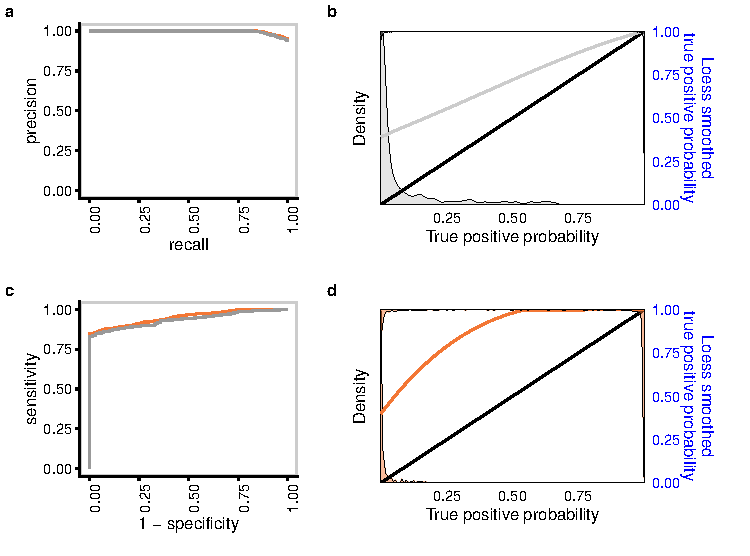
\includegraphics{figures/aml_plot.pdf}
%   \end{center}
%   \caption{Model performance on 300X Whole leukemia genome.
%   \textbf{(a)} Precision/recall curves and \textbf{(c)} Reciever operating characteristic curves.
%   Distribution of estimated true positive probabilities for true positive (top) and true negative (bottom) variants for \textbf{b)} the MuTect model and \textbf{d)} the Calibrated model.
%   A perfectly calibrated model would generate the diagonal line.}
%   \label{NAR-aml}
% \end{figure*}
\begin{figure*}
  \begin{center}
  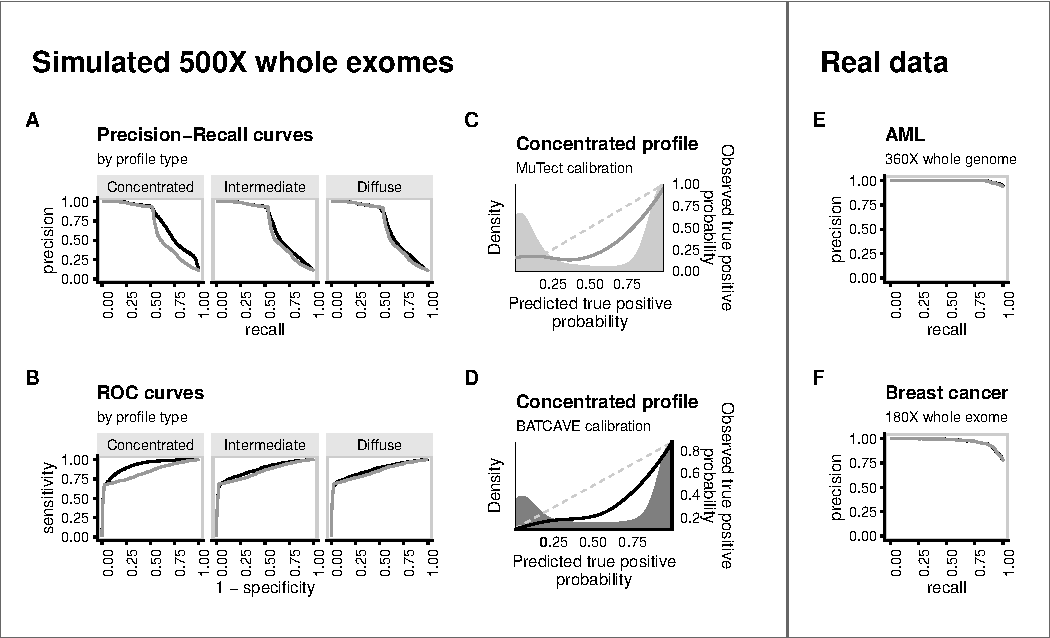
\includegraphics{figures/fig_wes.pdf}
  \end{center}
  \caption{Model performance on 500X simulated whole exome.
  \textbf{(a)} Precision recall curves and \textbf{(c)} Reciever operating characteristic curves for 3 mutation signatures.
  Distribution of estimated true positive probabilities for true positive (top) and true negative (bottom) variants for \textbf{b)} the MuTect model and \textbf{d)} the \batcave model.
  A perfectly calibrated model would generate the diagonal line.\bkmcomment{change the axis on b and d to be the same as the steyerberg paper. much clearer}}
\label{NAR-wes_fig}
\end{figure*}

\subsection{Simulated data}
We generated six different tumor/normal pairs of two types, 3 each of 100X depth whole genomes and 500X whole exomes.
For each of the two types we simulated tumors with variants drawn from three different mutation profiles (Concentrated,Intermediate, and Diffuse) as described in Materials \& Methods and Figure \ref{NAR-sigfig}.
These 6 simulated tumor/normal pairs were used to assess the effect of sequencing depth and mutation profile type on the results obtained from \batcave.
\bkmcomment{Should there be a longer discussion of what sorts of tumors the profiles represent, or leave that for the methods only?}

We assessed classification performance with both the area under the ROC curve and the area under the precision-recall curve, because the classes here are deeply unbalanced.
By both metrics \batcave outperforms MuTect (Figure \ref{NAR-wes_fig} \textbf{a} and \textbf{c}, and Table \ref{table:01}).
The extent to which \batcave outperforms is dependent on both the sequencing depth and the level of concentration of the mutation signature.
Deeper sequencing and more concentrated mutation signatures increase the performance advantage of \batcave. 

The estimated effective mutation rate, $\mu/\beta$, is in the range of 3e-7 for all simulated tumors.
We note that the effective mutation rate is lower than the simulated rate of 3e-6.
In this case the lower effective rate is not due to normal contamination of the tumor sample, but the fact that \texttt{Bamsurgeon} has restrictions -- such as sequencing depth and quality -- that prevent 100\% of simulated variants from being inserted. 
\bkmcomment{possible to quantify that this is very close to the actual insertion rate. Do it}.

We measured calibration performance using the Integrated Calibration Index described in Methods \citep{Austin2019}.
For all simulated tumors the calibration of \batcave is better across the full spectrum of posterior probabilities.
As we can see in Figure \ref{NAR-wes_fig} \textbf{b} and \textbf{d}, \batcave tends to increase posterior probabilities of low probability but true variants (top density curves), and decrease the probability of low probability but false variants (bottom density curves.).
As with all other metrics, the benefit of \batcave increases as the concentration of the mutation profile increases, and as sequencing depth increases.

The context-dependent prior probability of mutation, the heart of \batcave, depends on the prior converging to a good representation of the data generating distribution within the set of high-confidence mutations.
We use the Kullback-Leibler divergence as a measure of the distance (or entropy difference) between the estimated prior and the actual simulated data generating distribution.
In Figure \ref{NAR-sigfig} \textbf{e} and \textbf{f} we order mutations by descending MuTect probability value, and compute the KL divergence between the prior after adding each mutation and the data generating distribution.
For both whole exome and whole genome the prior converges to the data generating distribution easily within the number of available high-confidence mutations. 

\subsection{Real tumor data.}
\bkmcomment{need to rework this figure. the template allows only one full width figure.}

\bkmcomment{add TPR/FPR at 1\% and 3\%?}


\begin{table*}[b]
\tableparts{%
\caption{This is a table with $\mu$, auroc, auprc, ICI, and maybe fraction called?}
\label{table:01}%
}{%
\begin{tabular*}{\textwidth}{@{}lllllllll@{}}
\toprule
Depth & Mutation profile & $\mu/\beta$ & AUROC & & AUPRC & & ICI & 
\\
& & (estimated) & MuTect & \batcave & MuTect & \batcave & MuTect & \batcave
\\
\colrule
100X whole genome & Concentrated & 3.6e-7 & .987 & .993 & .972 & .975 & -- & --
\\
100X whole genome & Intermediate & 3.2e-7 & .987 & .989 & .972 & .973 & -- & --
\\
100X whole genome & Diffuse & 3.2e-7 & .988 & .989 & .971 & .973 & -- & --
\\
500X whole exome & Concentrated & 3.6e-7 & .848 & .929 & .674 & .758 & .0585 & .0462
\\
500X whole exome & Intermediate & 3.6e-7 & .847 & .881 & .677 & .706 & .0587 & .0568 
\\
500X whole exome & Diffuse & 3.6e-7 & .850 & .873 & .676 & .698 & .0565 & .0576
\\
AML 31 & Actual & 3.6e-8 & .935 & .949 & .995 & .996 & 0.121 & 0.155
\\
\botrule
\end{tabular*}%
}
{$\mu$ = per-base mutation rate, AUROC/AUPRC = area under ROC/PRC curve, ICI = Integrated calibration index.}
\end{table*}


\section{DISCUSSION}

-- Simulations suggest that if the mutation profile is the data generating distribution, \batcave can estimate effective mutation rate and data generating distribution, and doing so improves both classification and calibration.

-- One hope is to enable higher confidence in low frequency alleles as sequencing depth increases. Depth seems to have a very large effect on performance i.e. results are more compelling for 500X wes than for 100x wgs, although if you do 100 wgs you will still benefit.
In other words sequence depth matters more performance wise than sequencing breadth if the only desire is to see low frequency alleles. No advantage is gained (after a certain depth) of adding variants(sites) by wgs sequencing.
\subsection{Discussion subsection one}



\section{CONCLUSION}

Text. Text. Text. Text. Text. Text. Text. Text. Text. Text. Text.
Text. Text. Text. Text. Text. Text. Text. Text. Text. Text. Text.
Text. Text. Text. Text. Text. Text. Text. Text. Text. Text. Text.
Text. Text. Text. Text. Text. Text. Text. Text. Text. Text. Text.
Text. Text. Text. Text. Text. Text. Text. Text. Text. Text. Text.
Text. Text. Text. Text. Text. Text. Text. Text. Text. Text. Text.
Text. Text. Text. Text. Text. Text. Text. Text. Text. Text. Text.
Text. Text. Text. Text. Text. Text. Text. Text. Text. Text. Text.
Text. Text. Text. Text. Text. Text. Text. Text. Text. Text. Text.
Text. Text. Text.


\section{ACKNOWLEDGEMENTS}

Text. Text. Text. Text. Text. Text. Text. Text. Text. Text. Text.
Text. Text. Text. Text.


\subsubsection{Conflict of interest statement.} None declared.




\bibliography{caller_paper}

\section{Supplementary Figures}

\begin{figure*}[t]
  \begin{center}
  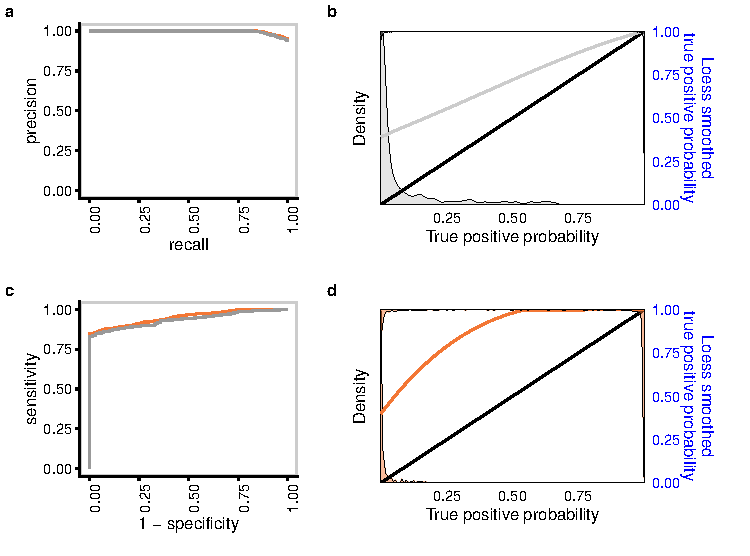
\includegraphics{figures/aml_plot.pdf}
  \end{center}
  \caption{Model performance on 300X Whole leukemia genome.
  \textbf{(a)} Precision/recall curves and \textbf{(c)} Reciever operating characteristic curves.
  Distribution of estimated true positive probabilities for true positive (top) and true negative (bottom) variants for \textbf{b)} the MuTect model and \textbf{d)} the Calibrated model.
  A perfectly calibrated model would generate the diagonal line.}
  \label{NAR-aml}
\end{figure*}

\begin{figure*}
  \begin{center}
  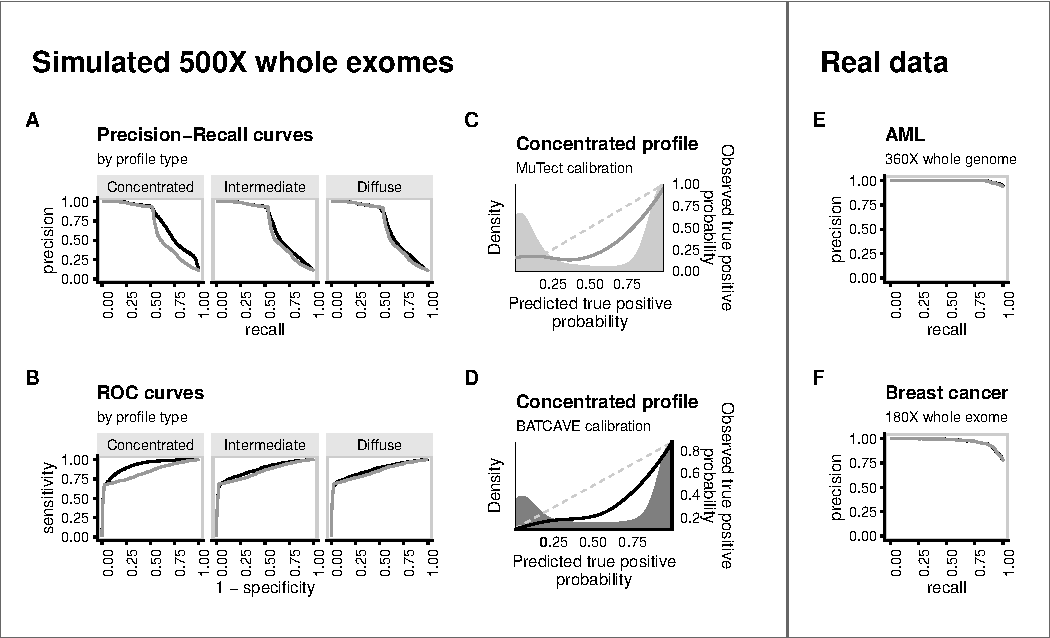
\includegraphics{figures/fig_wes.pdf}
  \end{center}
  \caption{Model performance on 100X simulated whole genome.
  \textbf{(a)} Precision recall curves and \textbf{(c)} Reciever operating characteristic curves for 3 mutation signatures.
  Distribution of estimated true positive probabilities for true positive (top) and true negative (bottom) variants for \textbf{b)} the MuTect model and \textbf{d)} the \batcave model.
  A perfectly calibrated model would generate the diagonal line.\bkmcomment{change the axis on b and d to be the same as the steyerberg paper. much clearer}}
\label{NAR-wgs_fig}
\end{figure*}
\end{document}
